%!TeX spellcheck=en_US
\documentclass[11pt,
               a4paper,
               bibtotoc,
               idxtotoc,
               headsepline,
               footsepline,
               footexclude,
               BCOR12mm,
               DIV13,
               openany,   % using this removes blank pages around part / chapter starts.
%               oneside    % include this if you have to print only one page per sheet of paper.
               ]
               {scrbook}

\include{settings}
\usepackage{lipsum} % for filling pages with stuff
\usepackage{tikz}
\usetikzlibrary{automata,positioning}
\usepackage[dvipsnames]{xcolor}

\lstdefinestyle{eclipse-rust} {
    captionpos=b,
    language=C++,
    otherkeywords={final},
    basicstyle=\footnotesize,
    numbers=left,
    numberstyle=\small,
    showstringspaces=false,
    tabsize=2,
    frame=single,
    breaklines=true,
    keywordstyle=\bfseries\color[RGB]{127,0,85},
    identifierstyle=\color[RGB]{0,0,192},
    stringstyle=\color[RGB]{42,0,255},
    commentstyle=\color[RGB]{63,127,95},
}
\lstdefinelanguage{Rust}{
    sensitive=true,
    morekeywords={as, break, const, continue, crate, else, enum, extern, false, fn, for, if, impl, in, let, loop, match, mod, move, mut, pub, ref, return, self, Self, static, struct, super, trait, true, type, unsafe, use, where, while, async, await, dyn, Result, Option, Ok, Err, panic},
    morecomment=[l]{//},
    morecomment=[s]{/*}{*/},
    morestring=[b]",
    morestring=[b]',
}

% -------------------------------------------------------------------------------
% --------------------------------- Thesis Info ---------------------------------
% -------------------------------------------------------------------------------

% set title, authors and stuff for the cover
% docytype needs xspace because it is used within text.
\def\doctype{Bachelor's Thesis\xspace}
%\def\doctype{Master's Thesis\xspace}
%\def\doctype{Guided Research\xspace}
%\def\doctype{Interdisciplinary Project\xspace}
\def\studyProgram{TUM School of CIT}
\def\title{Comparing Molecular Dynamics Simulations with Rust and C++}
% don't try translate every technical term if it would sound off
\def\titleGer{Unterschiede der Molekulardynamik Simulationen bei Rust und C++}
\def\author{Anatoly Weinstein}
% Prof
\def\supervisor{Univ.-Prof. Dr. Hans-Joachim Bungartz}
% PhD Candidate
\def\advisor{Markus Mühlhäußer, M. Sc.}
\def\date{24th August 2026}

\begin{document}
\frontmatter
% -------------------------------------------------------------------------------
% ---------------------------------- COVERPAGE ----------------------------------
% -------------------------------------------------------------------------------

% correct BCOR - undo at the end !!!
\def\bcorcor{0.15cm}
\addtolength{\hoffset}{\bcorcor}
\thispagestyle{empty}
\vspace{4cm}
\begin{center}
    \includegraphics[width=4cm]{templateStuff/tumlogo.pdf}\\[5mm]
    \huge SCHOOL OF COMPUTATION, INFORMATION AND TECHNOLOGY\\[5mm]
    \large DER TECHNISCHEN UNIVERSITÄT MÜNCHEN\\[24mm]

    {\Large \doctype in \studyProgram}\\[20mm]
    {\huge\bf \title\par}
    \vspace{15mm}
    {\LARGE  \author}
\end{center}

\cleardoubleemptypage

% -------------------------------------------------------------------------------
% ---------------------------------- TITLEPAGE ----------------------------------
% -------------------------------------------------------------------------------

\def\bcorcor{0.15cm}
\addtolength{\hoffset}{\bcorcor}
\thispagestyle{empty}
\vspace{10mm}
\begin{center}
    \includegraphics[width=4cm]{templateStuff/tumlogo.pdf}\\[5mm]
	\huge SCHOOL OF COMPUTATION, INFORMATION AND TECHNOLOGY\\[5mm]
	\large DER TECHNISCHEN UNIVERSITÄT MÜNCHEN\\[24mm]
	{\Large \doctype in \studyProgram}\\[20mm]
	{\LARGE\bf \title}\\[10mm]
	{\LARGE\bf \titleGer}\\[10mm]
	\begin{tabular}{ll}
		\Large Author:      	& \Large \author \\[2mm]
		\Large Supervisor:  	& \Large \supervisor\\[2mm]
		\Large Advisor:			& \Large \advisor\\[2mm]
		\Large Date:       		& \Large \date
	\end{tabular}
\end{center}

% undo BCOR correction
\addtolength{\hoffset}{\bcorcor}
\newpage

% -------------------------------------------------------------------------------
% ---------------------------------- DISCLAIMER ---------------------------------
% -------------------------------------------------------------------------------

\cleardoubleemptypage

\thispagestyle{empty}
\vspace*{0.7\textheight}
\noindent
I confirm that this \MakeLowercase{\doctype} is my own work and I have documented all sources and material used.\\

\vspace{15mm}
\noindent
Munich, \date \hspace{5cm} \author
\cleardoubleemptypage

% -------------------------------------------------------------------------------
% ------------------------------- ACKNOWLEDGEMENTS ------------------------------
% -------------------------------------------------------------------------------

\phantomsection
\addcontentsline{toc}{chapter}{Acknowledgements}
\vspace*{2cm}
\begin{center}
    {\Large \bf Acknowledgements}
\end{center}
\vspace{1cm}

I acknowlege everyone who has been with me on this journey and major milestone of my life, my sincerest Thank You to

My Family, who has been always with me, sponsored my education and gave me the opportunity to become who I am today.

My Friends, who were always there for me, who gave me the energy and motivation to continue to study. I especially credit Faid Rihan, Niklas Feurstein, Anna Lena Müller, Samhitha Girish Jois, Roman Danylchuk, Kirill Tikhomirov, Kameswara Siddharth Sishta, Kacper Darowski, Lucy Yang, Joana Arguirova, Junguo (Ryan) Xu, Melisa Aslan, Jongtae (Jerry) Park, Patrick Dirks.

My advisor, Markus Mühlhäußer, who is an amazing teacher and a great mentor. Without him I would not be able to organize my thesis into smaller scopes and probably would have moved most of the workload into the deadline week.

My bestie Kasane Teto, who has not said a word but always morally supported me with her inanimate gaze.



\cleardoublepage

% -------------------------------------------------------------------------------
% ---------------------------------- ABSTRACT -----------------------------------
% -------------------------------------------------------------------------------

\phantomsection
\addcontentsline{toc}{chapter}{Abstract}
\vspace*{2cm}
\begin{center}
    {\Large \bf Abstract}
\end{center}
\vspace{1cm}

\lipsum[2]

\cleardoublepage

\phantomsection
\addcontentsline{toc}{chapter}{Zusammenfassung}
\vspace*{2cm}
\begin{center}
    {\Large \bf Zusammenfassung}
\end{center}
\vspace{1cm}

\lipsum[2]

\cleardoublepage

% -------------------------------------------------------------------------------
% ------------------------------ TABLE OF CONTENTS ------------------------------
% -------------------------------------------------------------------------------

\tableofcontents
\thispagestyle{empty}
\cleardoubleemptypage

% -------------------------------------------------------------------------------
% --------------------------------- MAIN MATTER ---------------------------------
% -------------------------------------------------------------------------------

\mainmatter
\part{Introduction and Background}
\chapter{Introduction}
% labels can be put almost anywhere and can be referencef from anywhere.
\label{sec:intro}

In 2025 the StackOverflow's developer survey has ranked Rust as the most admired programming language, holding the title consecutively for nine years\cite{stackoverflow-technology-admired-and-desired}.

% https://survey.stackoverflow.co/
% https://survey.stackoverflow.co/2025/technology#admired-and-desired
% https://survey.stackoverflow.co/2024/technology#admired-and-desired
% https://survey.stackoverflow.co/2023#section-admired-and-desired-programming-scripting-and-markup-languages
% https://survey.stackoverflow.co/2022#technology-most-loved-dreaded-and-wanted
% https://survey.stackoverflow.co/2021#technology-most-loved-dreaded-and-wanted
% https://survey.stackoverflow.co/2020#most-loved-dreaded-and-wanted
% https://survey.stackoverflow.co/2019#most-loved-dreaded-and-wanted
% https://survey.stackoverflow.co/2018#most-loved-dreaded-and-wanted
% https://survey.stackoverflow.co/2016#technology
\vspace{1.5em}
\begin{figure}[h!]
\begin{tikzpicture}
    \begin{axis}[
        width=0.7\textwidth,  
        height=0.3\textheight,
        xlabel={Year},
        % ylabel={Percentage},
        ylabel={Percentage Admired},
        xtick={2010, 2015, 2020, 2025},
        scaled x ticks=false,  
        scaled y ticks=false,
        ymajorgrids=true, 
        grid style=dashed,
        ymin=-5,
        ymax=105,
        xmin=2014,
        xmax=2026,
        x tick label style={/pgf/number format/.cd, 1000 sep={}},
        % legend style={at={(0.02,0.45)},anchor=north west},
        legend style={at={(0.07,0.35)},anchor=north west},
    ]

    \addplot[
        color=blue,
        mark=square,
        line width=1pt,
        ]
        coordinates {
            (2015, 75.6)(2017, 52.0)(2018, 46.7)(2019, 52.0)(2020, 43.4)(2021, 49.2)(2022, 48.4)(2023, 49.8)(2024, 53.1)(2025, 46.6)
        };

    \addplot[
        color=Bittersweet,
        mark=triangle,
        line width=1pt,
        ]
        coordinates {
            (2015, 73.8)(2016, 79.1)(2017, 73.1)(2018, 78.9)(2019, 83.5)(2020, 86.1)(2021, 86.9)(2022, 86.7)(2023, 84.7)(2024, 82.2)(2025, 72.4)
        };

    % \addplot[
    %     color=cyan,
    %     mark=square,
    %     line width=1pt,
    %     ]
    %     coordinates {
    %         (2023, 16.4)(2024, 18.3)(2025, 16.7)
    %     };

    % \addplot[
    %     color=Dandelion,
    %     mark=triangle,
    %     line width=1pt,
    %     ]
    %     coordinates {
    %         (2023, 30.6)(2024, 28.7)(2025, 29.9)
    %     };

    \legend{C++, Rust}
    % \legend{C++ (Admired), Rust (Admired), C++ (Desired), Rust (Desired)}
    \end{axis}
\end{tikzpicture}
\caption{Rust and C++ in StackOverflows' survey on most admired programming languages}
\label{fig:stackoverflow-most-admired}
\end{figure}

In 2020, the social platform Discord had already published several blogposts explaining that they are rewritting software components in Rust\cite{discord-moves-to-rust}. Their main reasoning behind this decision was mostly about reaching high performance demands, but also about Rusts' type system which contrary to functional programming languages allowed mutation.

Specifically the blogpost mentions issuesses with the garbage collector of the Go Programming Language, which was rescanning the entire LRU cache for memory which can be freed, causing to latency spikes every 2 minutes.

% The same year on 18th November, the technology company Cloudflare ``began experiencing significant failures to deliver core network traffic''\cite{cloudflare-outage}, with Rust being featured as part of the error in the blogpost, creating a lot online discussions about the languages' relevance.

% The error was discovered to be with their Bot Management System. This software routes traffic and to do so it reads a `feature file' to stay in sync with an updated list of cyber attacks.
% A change to Cloudflares' database permissions caused the `feature file' to be written with duplicated rows.
% The Rust proxy-service, which had limited memory allocated, then became the source of the unhandled error when the feature file size grew three times larger than expected.

In 2024, Google has published a security blogpost with the topic on making their software memory safe, in which they mentioned a new migration approach called ``interoperability'' which offers an incremental approach to adopting memory safety in software\cite{google-eliminating-memory-safety-vulnerabilities}. This allows working on a multi-lingual codebase where new code is written in Rust, allowing the team to define their own pace of migrating to Rust.

This paper takes the goal of diving deeper into a more direct and technical comparison between Rust and C++ by writing a molecular dynamics simulation program in both programming languages and analyze the differences in usability and benchmark performance.

\chapter{Comparing Rust against C++}
\section{The Rust Ecosystem}

Before diving into the the syntax and the defining elements of the Rust Programming Language, this section will give a brief overview over the tooling and console applications provided by Cargo, the Rust Package Manager.

Since Cargo can install dependencies it was also designed to be extensible, meaning that most operations you will need to maintain a Rust project are located behind a Cargo subcommand.

\begin{description}
    \item[cargo run] Equivalent to \texttt{make run}, Cargo will invoke the Rust compiler on the codebase and execute the resulting binary.
    \item[cargo build] Equivalent to \texttt{make}, Cargo will invoke the Rust compiler on the codebase and compile a binary but not execute it.
    \item[cargo test] Equivalent to \texttt{ctest} or GoogleTest, Cargo has an integrated testing tool which will compile the codebase and run all functions annotated with \texttt{\#[test]} as an individual, isolated test case.
    \item[cargo doc] Equivalent to \texttt{Doxygen} or other documentation libraries, Cargo provides an in-built way of generating documentation for the codebase.
    \item[cargo fmt] Equivalent to \texttt{clang-format}, Cargo provides an in-built way to format the entire codebase.
    \item[cargo clippy] Equivalent to \texttt{clang-tidy}, Cargo provides an in-built way to lint and statically analyze the codebase. This command is also often used in CI/CD to ensure the codebase quality.
\end{description}

The first difference observation in terms of usability is that the C++ infrastructure is fragmented, whereas for Rust it is centralized via its package manager. This smoothes down the learning curve of Rust tools, as new users only have to get comfortable with one tool, which incorporates 

It's noteworthy to mention that there's no equivalent to GDB in the Rust ecosystem because the type system and ownership model of Rust guaranteee safety over memory and thread.

\section{The Rust Programming Language}

% Rust has two `modes' in which code can be written. The more commonly used one is called `Safe Rust' which can be statically analysed and is guaranteed not to cause segmentation faults and core dumps, and the one with extra powers is called `Unsafe Rust'.

% `Unsafe Rust' are scopes and functionalities marked with the keyword \texttt{unsafe} which allow for example mutating static variables, dereferencing pointers and invoking other unsafe functionalities\cite{rust-book-unsafe-rust}. We will not dive deeper into Unsafe Rust than just mention it as it is mostly off-topic to this thesis.

% We will now look at the syntax of `Safe Rust'.

\subsection{Syntax}

It's always better to see the syntax than get it explained, so in the figure below you can see an example.

Compared to C++, the main syntactical difference in Rust is that the type always follows the variable, attribute and function argument and not preceeds it. 

TODO

\subsection{Structs and Traits}

Structs in Rust are almost entirely equivalent to C++ structs. A struct is a type which defines a collection of fields. Unlike in C++ however, Rust has no concept of struct inheritance. Instead of abstract classes, Rust provides traits, which is an abstract interface that types can implement explicitly.

% \vspace{1.5em}
% \setlength{\columnsep}{2em}
% \begin{multicols}{2}
% \begin{lstlisting}[style=eclipse-cpp, caption=An abstract class in C++, label=code:cpp-abstract-class]
% class Force {
%     virtual double potential(const Particle &particle, const Particle &other) const;
% }
% \end{lstlisting}

% \vfill\null
% \columnbreak

% \begin{lstlisting}[style=eclipse-rust, language=Rust, basicstyle=\ttfamily\small, caption=A Trait definition in Rust, label=code:rust-trait]
% pub trait Force {
%     fn potential(&self, particle: &Particle, other: &Particle) -> f64;
% }
% \end{lstlisting}

% \begin{lstlisting}[style=eclipse-rust, language=Rust, basicstyle=\ttfamily\small, caption=An implementation of the Force trait in Rust, label=code:rust-trait-implement]
% impl Force for NewtonForce {
%     fn potential(&self, particle: &Particle, other: &Particle) -> f64 {

%     }
% }
% \end{lstlisting}
% \end{multicols}

In C++ a class can only inherit from one `abstract class'. An abstract class is From a developer

Todo!

\subsection{Ownership Model}

Todo!

\subsection{Dynamic Dispatch}

Both the C++ and Rust implementations use dynamic dispatch. 

\subsection{Error Handling}

Option, Result and Panic

\subsection{Unsafe Rust}

What we have learned so far has been `Safe Rust', which can be statically analyzed for memory safety and bugs that would cause segmentation fault in C++ are caught in the compilation stage.

However sometimes because of performance reasons or communicating with an external library, code has to be written using of raw pointer arithmetics. This mode is commonly referred to as `Unsafe Rust'.

An unsafe functionality is a scope, function or trait implementation annotated with the \texttt{unsafe} keyword. In an unsafe block, Rust gives you access to a few operations which can not be statically verified and could cause undefined behaviour. The operations are the following.

\begin{enumerate}
    \item Dereferencing a pointer.
    \item Using other unsafe functionalities like invoking an unsafe function or implementing an unsafe trait.
    \item Read or write to a mutable static variable.
    \item Accessing fields of a \texttt{union}, a special element which is syntactically similar to a struct with the exception of all fields sharing the same storage.
\end{enumerate}

To get a bit of intuition on what kind of operations are unsafe consier this example: For a struct to be shared accross threads, it needs to implement the \texttt{Sync} trait, which is unsafe. If the struct also contains a pointer which you would like to interpret at index $2$, adding $2$ to the pointer and dereferencing it is also unsafe behaviour.

\subsection{Macros}

rust macros vs c++ templates

\section{Compiler Error Messages}

mention how rusts' compiler error messages differ from C++

% \chapter{Rust Project Quickstart}

\section{Major Dependencies in Rust}

Below are two creditworthy libraries which are utilized in the project and severely improve the programming workflow. They utilize procedural macros to generate code from a struct.

\subsection{Clap}

clap

\subsection{Serde}

serde

\subsection{Rayon}

serde

\chapter{Application with Molecular Dynamics}

talk briefly about the physics

\chapter{Methods and Implementation}

talk about project infrastructure

\section{Molecular Dynamics Simulation}

\subsection{Program Frame}

talk about core implementation: core, io, cli

\subsection{Core Library}

talk about core implementation: core, io, cli

\subsection{I/O Library}

talk about core implementation: core, io, cli

\subsection{Parallelization in Rust}

\section{Benchmarking CI}

talk about automatic equality tester and benchmark CI script 

\section{External Tools}

talk about perf

\part{Evaluation}

\chapter{Benchmarking}

All following benchmarks are executed on a 64-bit 12th Gen Intel(R) Core(TM) i7-12700K. It has 12 cores and 20 logical CPU threads\cite{cpu-benchmark-intel-core-i7-12700k}, the particle dataset \texttt{two-bodies-collision} is used for benchmarking, which moves a $20 \times 20$ matrix of particles against a $100 \times 20$ wall of particles, creating a dataset of $2,400$ particles. The statistics below were measured as ``the average of 20 runs'' of the x-axis value.

Despite being two-dimensional input, the computational complexity of the algorithms remains identical, with \texttt{DirectSum} iterating over all particle pairs and \texttt{LinkedCells} only over neighbouring cells. The measured performance should also not change much because it is dominated by loop structure, and adding the z-axis to \texttt{LinkedCells} is a minimal change in comparison.

For interested readers we will provide some further benchmarks (including 3D benchmarks) in the Appendix but not cover it in this section.

\section{Sequential}

\vspace{1.5em}
\begin{figure}[h!]
\begin{tikzpicture}
    \begin{axis}[
        width=0.7\textwidth,  
        height=0.3\textheight,
        xlabel={Simulation Steps},
        ylabel={Average Time (ms)},
        xtick={0, 100, 200, 300, 400, 500},
        ytick={0, 2000, 4000, 6000, 8000, 10000},
        scaled x ticks=false,  
        scaled y ticks=false,
        ymajorgrids=true, 
        grid style=dashed,
        % ymin=-10,
        % xmin=-5,
        x tick label style={/pgf/number format/.cd, 1000 sep={}},
        legend style={at={(0.02,0.98)},anchor=north west},
    ]

    \addplot[
        color=blue,
        mark=square,
        mark repeat={10},
        mark phase={10},
        line width=1pt,
        ]
        coordinates {
            (10, 273.8165997)
            (20, 516.9802851000001)
            (30, 740.55466115)
            (40, 937.56702935)
            (50, 1155.55535655)
            (60, 1370.89085105)
            (70, 1590.08775205)
            (80, 1804.2172272999999)
            (90, 2025.46045965)
            (100, 2216.8778125)
            (110, 2431.91059725)
            (120, 2647.86904725)
            (130, 2874.7884709)
            (140, 3081.6999533499998)
            (150, 3299.1595616)
            (160, 3517.76840055)
            (170, 3740.72414485)
            (180, 3987.1059080500004)
            (190, 4178.9094133)
            (200, 4394.18286335)
            (210, 4615.9988649)
            (220, 4830.2009383)
            (230, 5033.0900034)
            (240, 5259.07758855)
            (250, 5475.493254)
            (260, 5696.6816693)
            (270, 5900.11267575)
            (280, 6128.872172)
            (290, 6351.41395755)
            (300, 6575.61442405)
            (310, 6782.6294163)
            (320, 6997.100106100001)
            (330, 7214.3388998)
            (340, 7420.6009662)
            (350, 7642.31302525)
            (360, 7876.449799149999)
            (370, 8077.65604555)
            (380, 8293.26344745)
            (390, 8508.0315137)
            (400, 8734.0040768)
            (410, 8950.470459350001)
            (420, 9174.05059475)
            (430, 9384.57252745)
            (440, 9638.45208945)
            (450, 9848.6973095)
            (460, 10044.4907458)
            (470, 10293.8542321)
            (480, 10476.38084845)
            (490, 10701.7011691)
            (500, 10917.5842851)
        };

    \addplot[
        color=Bittersweet,
        mark=triangle,
        mark repeat={10},
        mark phase={10},
        line width=1pt,
        ]
        coordinates {
            (10, 206.09075190000001)
            (20, 420.86882985)
            (30, 609.5883635499999)
            (40, 784.47083405)
            (50, 972.9397255499999)
            (60, 1160.30990525)
            (70, 1350.95556955)
            (80, 1539.5883787)
            (90, 1729.51311195)
            (100, 1901.3169879000002)
            (110, 2087.1569292)
            (120, 2278.9023803)
            (130, 2468.1327925)
            (140, 2652.2499233000003)
            (150, 2840.19161545)
            (160, 3024.94122365)
            (170, 3213.6127385)
            (180, 3406.8531513000003)
            (190, 3597.93581975)
            (200, 3786.7982349)
            (210, 4033.17009595)
            (220, 4191.15093275)
            (230, 4338.96322725)
            (240, 4536.2946618000005)
            (250, 4720.02117385)
            (260, 4911.74336795)
            (270, 5100.7897686999995)
            (280, 5281.31964145)
            (290, 5475.7793846)
            (300, 5669.91193965)
            (310, 5901.7394782)
            (320, 6039.34020995)
            (330, 6228.61913715)
            (340, 6407.84774325)
            (350, 6613.3648029)
            (360, 6791.39326845)
            (370, 6978.2380791000005)
            (380, 7175.9149278)
            (390, 7354.5108424499995)
            (400, 7551.263935399999)
            (410, 7733.4011731499995)
            (420, 7924.4063864)
            (430, 8122.7348954)
            (440, 8329.46436305)
            (450, 8498.965259300001)
            (460, 8693.306484)
            (470, 8885.7254749)
            (480, 9067.0104245)
            (490, 9255.374591950002)
            (500, 9456.65880155)
        };

    \addplot[
        color=cyan,
        mark=square,
        mark repeat={10},
        mark phase={10},
        line width=1pt,
        ]
        coordinates {
            (10, 78.3857747)
            (20, 97.78689784999999)
            (30, 118.27043359999999)
            (40, 139.91425819999998)
            (50, 159.9777254)
            (60, 181.944428)
            (70, 202.05761130000002)
            (80, 223.32035184999998)
            (90, 244.2928691)
            (100, 263.0832976)
            (110, 283.12121175)
            (120, 304.12945855000004)
            (130, 326.40458865)
            (140, 347.4012806)
            (150, 367.6449568)
            (160, 390.13839665)
            (170, 412.33240285000005)
            (180, 431.96820660000003)
            (190, 454.40316745)
            (200, 476.21270665)
            (210, 496.58448505)
            (220, 518.2896354)
            (230, 540.023347)
            (240, 559.3948907)
            (250, 581.7028173)
            (260, 603.4115296)
            (270, 626.28614905)
            (280, 648.1188669)
            (290, 656.43423115)
            (300, 674.7154297000001)
            (310, 697.06193475)
            (320, 718.2341502999999)
            (330, 740.2827422)
            (340, 761.22161135)
            (350, 782.7719842)
            (360, 805.83930565)
            (370, 826.1259000499999)
            (380, 848.58010345)
            (390, 869.51216685)
            (400, 892.1319427000001)
            (410, 913.1511605)
            (420, 932.2080336)
            (430, 955.71607565)
            (440, 978.6182835)
            (450, 1009.3205958)
            (460, 1024.3454271)
            (470, 1043.1995734)
            (480, 1065.2741108999999)
            (490, 1090.15862325)
            (500, 1108.8267938)
        };

    \addplot[
        color=Dandelion,
        mark=triangle,
        mark repeat={10},
        mark phase={10},
        line width=1pt,
        ]
        coordinates {
            (10, 28.013442050000002)
            (20, 48.023687100000004)
            (30, 65.20919214999999)
            (40, 81.64149454999999)
            (50, 98.8272592)
            (60, 114.3483536)
            (70, 132.27922695)
            (80, 149.11345219999998)
            (90, 166.00965965)
            (100, 178.76147815000002)
            (110, 194.35375275)
            (120, 211.73683935)
            (130, 228.51652615)
            (140, 245.5042519)
            (150, 261.61059385)
            (160, 279.19483825)
            (170, 295.67724695)
            (180, 313.23755255000003)
            (190, 330.21416165)
            (200, 346.37079935)
            (210, 362.80136555)
            (220, 380.05870830000003)
            (230, 411.41355265)
            (240, 414.25709345)
            (250, 435.87884994999996)
            (260, 458.97159545)
            (270, 476.02770625)
            (280, 493.43407035)
            (290, 502.29934195)
            (300, 520.41695385)
            (310, 554.5337899)
            (320, 565.9049047000001)
            (330, 583.9541938)
            (340, 589.600479)
            (350, 608.392485)
            (360, 625.04884805)
            (370, 643.18865175)
            (380, 659.46755515)
            (390, 677.32664225)
            (400, 695.7386448999999)
            (410, 712.75113485)
            (420, 730.49943815)
            (430, 747.7464812999999)
            (440, 766.51917615)
            (450, 783.7218594)
            (460, 801.9372038500001)
            (470, 818.69841815)
            (480, 837.5274133500001)
            (490, 854.6188709500001)
            (500, 871.80830505)
        };

    \legend{C++ [DirectSum], Rust [DirectSum], C++ [LinkedCells], Rust [LinkedCells]}
    \end{axis}
\end{tikzpicture}
\caption{Rust and C++ sequential performance on a ``two bodies collision'' input.}
\label{fig:benchmark-sequential}
\end{figure}

For the DirectSum implementation, when measuring sequential performance against simulation steps $S$ and other configuration data fixed, we observe linear runtime $\mathcal{O}(S)$. This is because, despite having to compute all particle pairs, the amount of particles $N$ and hence the workload per simulation step is constant in this graph.

To ensure the credibility of the computed average, the fluctuations between minimal and maximal run duration have also been recorded.
% The biggest relative outlier occured with Rust at 210 steps with a fluctuation of $20.9\%$.
A massive absolute outlier occured with Rust at the 310 steps benchmark, with a measured fluctuation of $435.6$ms or $7.4\%$. Fluctuations can be perceived in the graph as small `bumps'. At 500 steps, the recorded fluctuation in measured performance for both Rust and C++ are below $0.4\%$.

We can therefore derive the following claim in regards to the sequential performance ratio: Rust DirectSum completes in $86.6\%$ of the time taken by the C++ DirectSum implementation, with a speedup of $15.5\%$.

\begin{figure}[h]
\begin{tikzpicture}
    \begin{axis}[
        width=0.7\textwidth,  
        height=0.3\textheight,
        xlabel={Simulation Steps},
        ylabel={Average Time (ms)},
        xtick={0, 100, 200, 300, 400, 500},
        ytick={0, 200, 400, 600, 800, 1000, 1200},
        scaled x ticks=false,  
        scaled y ticks=false,
        ymajorgrids=true, 
        grid style=dashed,
        % ymin=-10,
        % xmin=-5,
        x tick label style={/pgf/number format/.cd, 1000 sep={}},
        legend style={at={(0.02,0.98)},anchor=north west},
    ]

    \addplot[
        color=cyan,
        mark=square,
        mark repeat={10},
        mark phase={10},
        line width=1pt,
        ]
        coordinates {
            (10, 78.3857747)
            (20, 97.78689784999999)
            (30, 118.27043359999999)
            (40, 139.91425819999998)
            (50, 159.9777254)
            (60, 181.944428)
            (70, 202.05761130000002)
            (80, 223.32035184999998)
            (90, 244.2928691)
            (100, 263.0832976)
            (110, 283.12121175)
            (120, 304.12945855000004)
            (130, 326.40458865)
            (140, 347.4012806)
            (150, 367.6449568)
            (160, 390.13839665)
            (170, 412.33240285000005)
            (180, 431.96820660000003)
            (190, 454.40316745)
            (200, 476.21270665)
            (210, 496.58448505)
            (220, 518.2896354)
            (230, 540.023347)
            (240, 559.3948907)
            (250, 581.7028173)
            (260, 603.4115296)
            (270, 626.28614905)
            (280, 648.1188669)
            (290, 656.43423115)
            (300, 674.7154297000001)
            (310, 697.06193475)
            (320, 718.2341502999999)
            (330, 740.2827422)
            (340, 761.22161135)
            (350, 782.7719842)
            (360, 805.83930565)
            (370, 826.1259000499999)
            (380, 848.58010345)
            (390, 869.51216685)
            (400, 892.1319427000001)
            (410, 913.1511605)
            (420, 932.2080336)
            (430, 955.71607565)
            (440, 978.6182835)
            (450, 1009.3205958)
            (460, 1024.3454271)
            (470, 1043.1995734)
            (480, 1065.2741108999999)
            (490, 1090.15862325)
            (500, 1108.8267938)
        };

    \addplot[
        color=Dandelion,
        mark=triangle,
        mark repeat={10},
        mark phase={10},
        line width=1pt,
        ]
        coordinates {
            (10, 28.013442050000002)
            (20, 48.023687100000004)
            (30, 65.20919214999999)
            (40, 81.64149454999999)
            (50, 98.8272592)
            (60, 114.3483536)
            (70, 132.27922695)
            (80, 149.11345219999998)
            (90, 166.00965965)
            (100, 178.76147815000002)
            (110, 194.35375275)
            (120, 211.73683935)
            (130, 228.51652615)
            (140, 245.5042519)
            (150, 261.61059385)
            (160, 279.19483825)
            (170, 295.67724695)
            (180, 313.23755255000003)
            (190, 330.21416165)
            (200, 346.37079935)
            (210, 362.80136555)
            (220, 380.05870830000003)
            (230, 411.41355265)
            (240, 414.25709345)
            (250, 435.87884994999996)
            (260, 458.97159545)
            (270, 476.02770625)
            (280, 493.43407035)
            (290, 502.29934195)
            (300, 520.41695385)
            (310, 554.5337899)
            (320, 565.9049047000001)
            (330, 583.9541938)
            (340, 589.600479)
            (350, 608.392485)
            (360, 625.04884805)
            (370, 643.18865175)
            (380, 659.46755515)
            (390, 677.32664225)
            (400, 695.7386448999999)
            (410, 712.75113485)
            (420, 730.49943815)
            (430, 747.7464812999999)
            (440, 766.51917615)
            (450, 783.7218594)
            (460, 801.9372038500001)
            (470, 818.69841815)
            (480, 837.5274133500001)
            (490, 854.6188709500001)
            (500, 871.80830505)
        };

    \legend{C++ [LinkedCells], Rust [LinkedCells]}
    \end{axis}
\end{tikzpicture}
\caption{Only the \texttt{LinkedCells} implementation from~\ref{fig:benchmark-sequential}}
\label{fig:benchmark-linked-cells}
\end{figure}

In figure~\ref{fig:benchmark-linked-cells} we can see the performance of specifically the LinkedCells implementation. The first thing that can be noticed is that the fluctuations are ``more noticable''. This is because as the graph is downscaled roughly 10 times on the y axis compared to figure~\ref{fig:benchmark-sequential}, a fluctuation of even 1ms is perceived ten times stronger.

We can derive the following further claims in regards to the sequential performance ratio: Rust LinkedCells completes in $78.6\%$ of the time taken by the C++ LinkedCells implementation, with a speedup of $27.2\%$.

Within the languages, we can derive the following claims in regards to choice of algorithm: Rust LinkedCells completes in $9.2\%$ of Rust DirectSum with a speedup of $1084.7\%$. C++ LinkedCells completes in $10.2\%$ of C++ DirectSum, with a speedup of $984.6\%$.

\newpage
\section{Parallel}

\begin{figure}[!htb]
\begin{tikzpicture}
    \begin{axis}[
        width=0.7\textwidth,  
        height=0.3\textheight,
        xlabel={Threads},
        ylabel={Average Time (ms)},
        xtick={1, 5, 10, 15, 20, 25, 30, 35, 40},
        ytick={0, 2000, 4000, 6000, 8000, 10000},
        scaled x ticks=false,  
        scaled y ticks=false,
        ymajorgrids=true, 
        grid style=dashed,  
        % ymin=-10,
        % xmin=-5,
        x tick label style={/pgf/number format/.cd, 1000 sep={}},
        legend style={at={(0.64,0.98)},anchor=north west},
    ]

    \addplot[
        color=blue,
        mark=square,
        mark repeat={10},
        mark phase={10},
        line width=1pt,
        ]
        coordinates {
            (1, 10549.44102935)
            (2, 5571.0913138000005)
            (3, 3828.3011744)
            (4, 2959.53039775)
            (5, 2453.5616619)
            (6, 2086.83681485)
            (7, 1872.2937152)
            (8, 1776.9810624000002)
            (9, 2842.05725815)
            (10, 2579.0881229)
            (11, 2237.2077405)
            (12, 2098.12427635)
            (13, 1945.8673943499998)
            (14, 1834.7854885)
            (15, 1737.7995877)
            (16, 1635.72036285)
            (17, 1548.6944922)
            (18, 1484.56652175)
            (19, 1410.4665424000002)
            (20, 1378.5975749000002)
            (21, 2886.65640485)
            (22, 2820.35793615)
            (23, 2570.67194405)
            (24, 2418.262331)
            (25, 2386.08754575)
            (26, 2306.1179389)
            (27, 2212.4575794499997)
            (28, 2085.6263195)
            (29, 1841.7964625999998)
            (30, 1776.5723484)
            (31, 1657.9944204)
            (32, 1630.8799666500001)
            (33, 1597.1685227)
            (34, 1561.5688749)
            (35, 1558.91068575)
            (36, 1581.21849395)
            (37, 1628.8673056)
            (38, 1715.87312205)
            (39, 1765.7758779)
            (40, 1790.1709173)
        };

    \addplot[
        color=Bittersweet,
        mark=triangle,
        mark repeat={10},
        mark phase={10},
        line width=1pt,
        ]
        coordinates {
            (1, 9658.2842576)
            (2, 4928.910334)
            (3, 3444.8674518000003)
            (4, 2587.9484446)
            (5, 2123.67822905)
            (6, 1860.88941835)
            (7, 1599.865377)
            (8, 1449.7257015)
            (9, 1346.69641615)
            (10, 1280.6119758)
            (11, 1219.16149855)
            (12, 1134.953047)
            (13, 1137.1112062)
            (14, 1124.4028151500002)
            (15, 1138.0777120999999)
            (16, 1138.08137515)
            (17, 1124.48505445)
            (18, 1124.25393865)
            (19, 1131.8717731)
            (20, 1134.6383659)
            (21, 1142.52283475)
            (22, 1149.5561255)
            (23, 1153.69549885)
            (24, 1171.25854415)
            (25, 1176.3205187)
            (26, 1184.5056304500001)
            (27, 1184.9608248499999)
            (28, 1202.0229382999999)
            (29, 1205.6641779000001)
            (30, 1207.92434495)
            (31, 1230.0749434000002)
            (32, 1227.61008325)
            (33, 1237.89594195)
            (34, 1251.675005)
            (35, 1264.6783749)
            (36, 1273.0318458499999)
            (37, 1251.2744953499998)
            (38, 1243.1092524)
            (39, 1260.36524855)
            (40, 1253.9120003)
        };

    \draw[dashed, red, line width=0.5pt] (axis cs:8.5,0) -- (axis cs:8.5,10000);
    \draw[dashed, red, line width=0.5pt] (axis cs:20.5,0) -- (axis cs:20.5,10000);

    \legend{C++ [OMP], Rust [Rayon]}
    \end{axis}
\end{tikzpicture}
\caption{Absolute strong scaling Rust and C++ performance on a ``two bodies collision'' input dataset, with 500 simulation steps executed with the parallel DirectSum implementation.}
\label{fig:benchmark-parallel}
\end{figure}

% Todo! x = thread, y = runtime (absolute [strong scaling] or relative [strong scaling speedup])

In the parallelized DirectSum implementation for both Rust and C++ we only parallelize the code segment which performs operations for every particle pair, by parallelizing the `outer' iteration and keeping the `inner' iteration sequential. We should also note here, that we don't really compare the capacities of the programming languages here, but of two specific parallelization libraries.

For Rust, we use Rayon as the parallelization library, and for C++ we use OMP. The thread count was set with environment variables \texttt{RAYON\_NUM\_THREADS} and \texttt{OMP\_NUM\_THREADS}.

The first difference we observe is that there are specific thread counts, where OMP performance drops. On the machine where the benchmarks were run, there was a 1066ms drop between thread counts 8 and 9, and a 1508ms drop between thread counts 20 and 21. This is probably because OMP takes the environment variable without further preprocessing and Rayon prefers the smaller of the environment variable and logical cores. The performance drop is marked with vertical dashed lines in figure~\ref{fig:benchmark-parallel}.

It's also noteworthy that above 20 threads, the the C++ implementation shows no stable performance pattern, this is most likely because at an overhead this high, the operating software dispatcher affects measurements.

At 2 threads, Rust parallel DirectSum completes in $88.5\%$ of the time taken by the C++ parallel DirectSum implementation, with a speedup of $22.6\%$. At 8 threads, Rust parallel DirectSum completes in $81.6\%$ of the time taken by the C++ parallel DirectSum implementation, with a speedup of $13\%$.

\chapter{Discussion and Conclusion}

discuss that rust is more usable, performs better, mention implementation bias (again)

conclude that you should not always switch to rust (rewrite tech debt, team skills and language learning logistics)

% template

\part{Template Stub (Remove)}

\chapter{Tips}
\subsection{How to Describe}
% optional: set the spacing between columns
\setlength{\columnsep}{30 pt}
When listing several points you have three basic options:
\begin{multicols}{3}
    \begin{itemize}
        \item itemize
        \item enumerate
        \item description
    \end{itemize}

    \vfill\null
    \columnbreak

    \begin{enumerate}
        \item itemize
        \item enumerate
        \item description
    \end{enumerate}

    \vfill\null
    \columnbreak

    \begin{description}
        \item[itemize] short, unordered
        \item[enumerate] short ordered
        \item[description] listing of descriptions. Also nice for longer ones.
    \end{description}

\end{multicols}


\subsection{How to Quote}

\begin{quote}
    "This is a quote!"
\end{quote}

\begin{itemize}
    \item Citations to a source can be made like this \verb|\cite{gratl17task}| =~\cite{gratl17task}
    \subitem Always join text and the citation with a non-breaking space: \verb|text~\cite{foo}|.
    \item Referencing Sections, Figures, Tables, Formulas: \verb|\autoref{sec:intro}| = \autoref{sec:intro}.
    \item Footnotes for url or further notes: \verb|\footnote{\url{https://www.top500.org}}| = \footnote{\url{https://www.top500.org}}
\end{itemize}

\subsection{How to Math}

Use the align environment for equations especially if you want to align them somehow.

\begin{align}
1 + 1 &\ne 3\\
\left(\dfrac{10}{1}\right) - 9 &= 1
\end{align}

% if you need a pagebreak because figure placement is broken:
\clearpage

\section{Environments}

\subsection{How to Figure}

Anything can also be put in multiple columns.

\begin{multicols}{2} % defines an environment with two columns
    \begin{figure}[H] % [H] for HERE
        \centering
        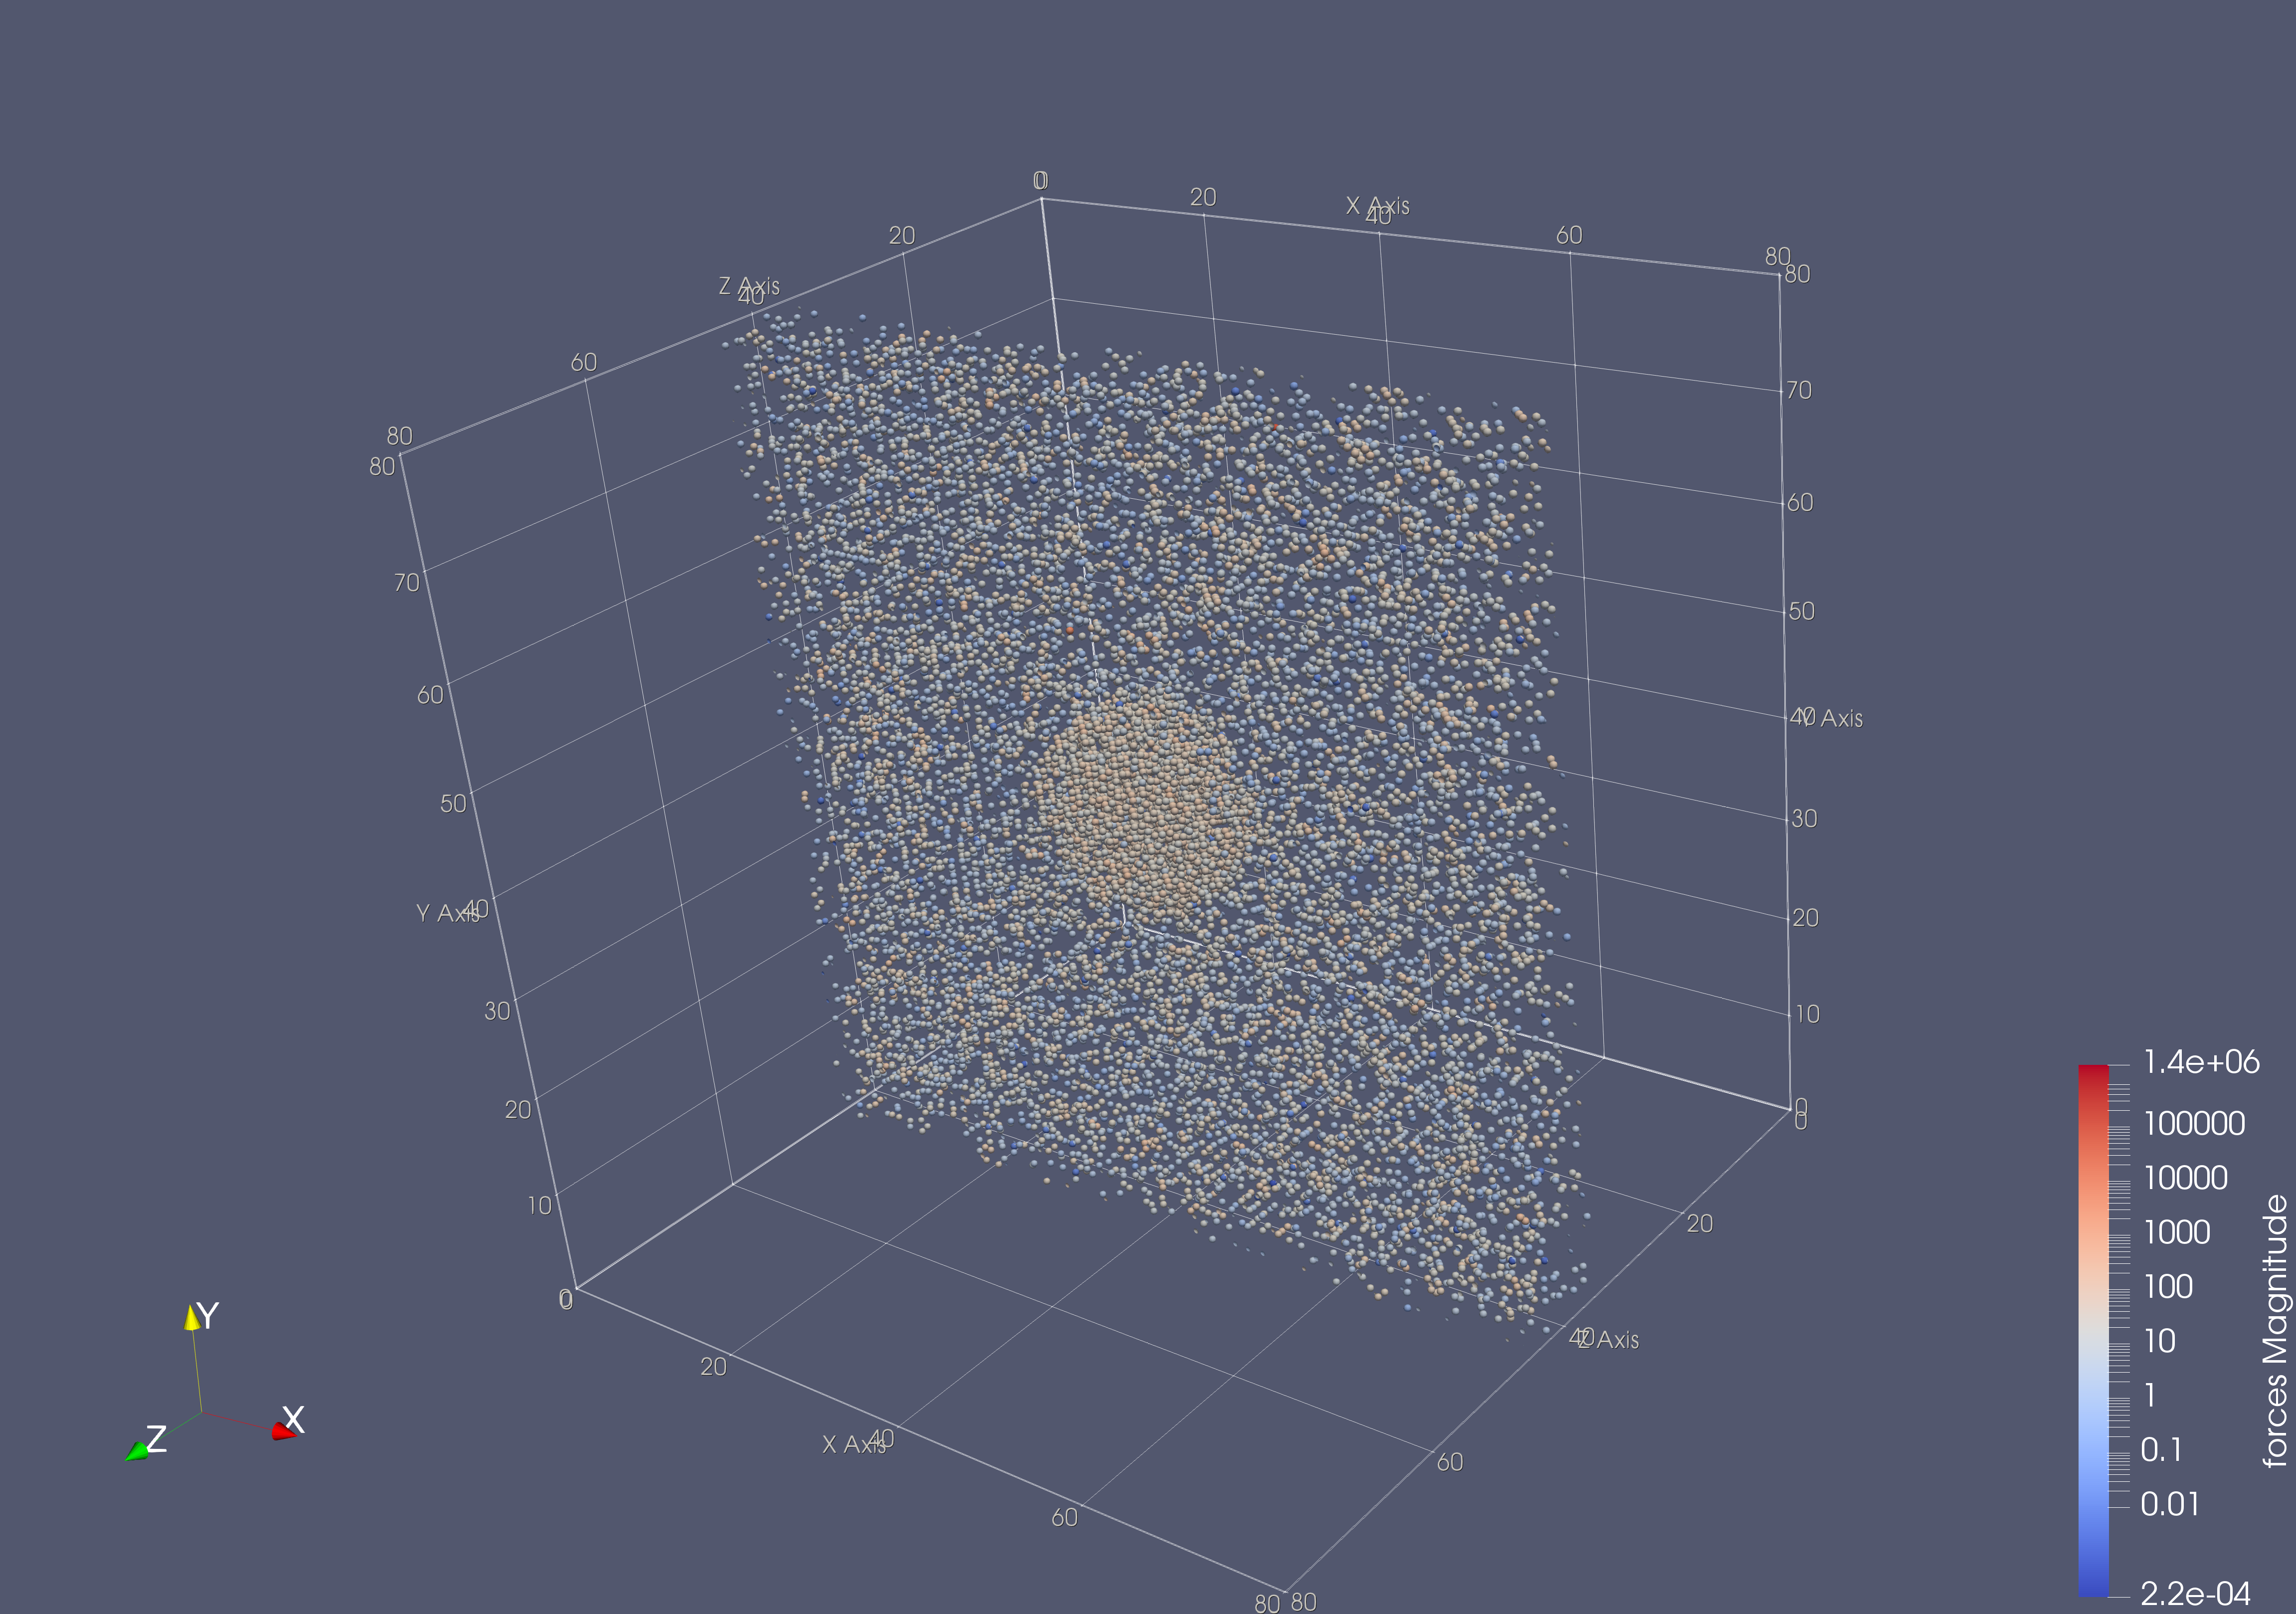
\includegraphics[width=.9\columnwidth]{figures/scenario_clip_rot.png}
        \caption[Example Figure]{Some Caption. Always also include a source if it wasn't created by you!\\
            \tiny{Source: \cite{gratl17task}}}
        \label{fig:exampleLabel1} % labels always have to be placed after the caption
    \end{figure}

    \columnbreak    % start next column

    \begin{figure}[H]
        \centering
        \begin{tikzpicture}
            \node[anchor=south west,inner sep=0] (image) at (0,0) {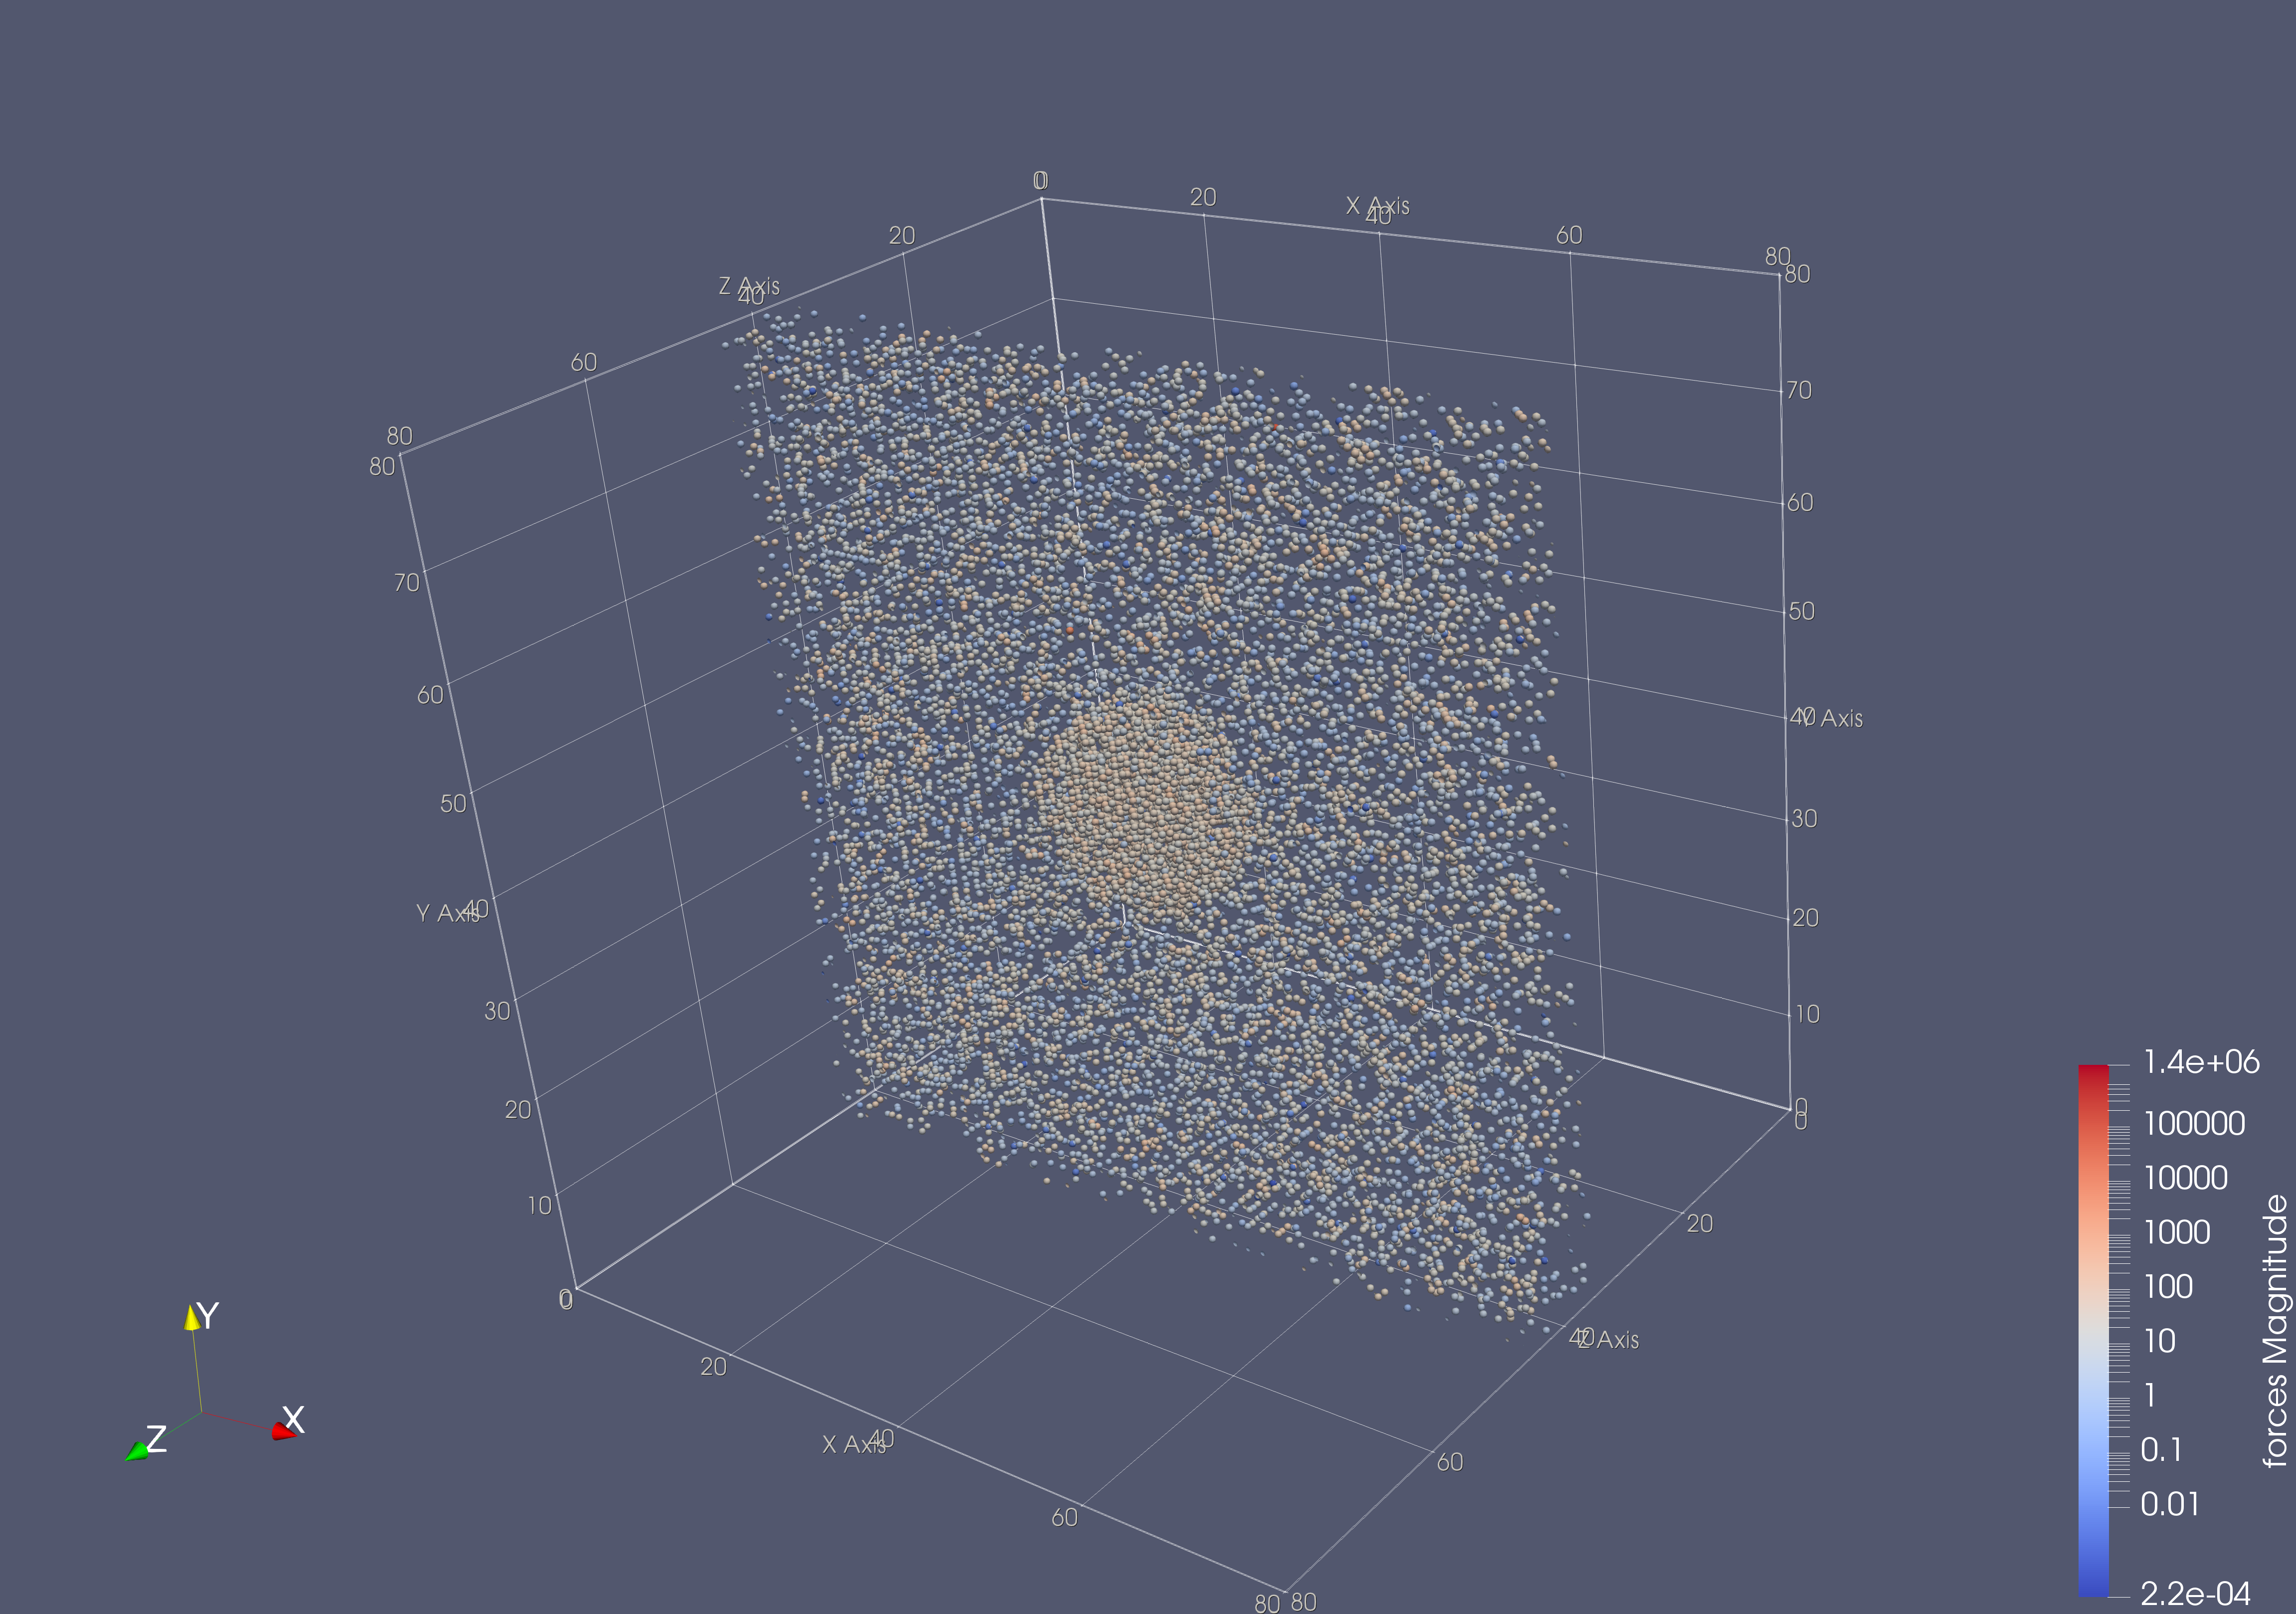
\includegraphics[width=.9\columnwidth]{figures/scenario_clip_rot.png}};
            \begin{scope}[x={(image.south east)},y={(image.north west)}]
            \draw[red, thin,rounded corners] (.42,.42) rectangle (.58,.6);
            \end{scope}
        \end{tikzpicture}
        \caption[Figure with tikz]{Figures can be drawn on or completely generated with tikz.}
        \label{fig:exampleLabel2}
    \end{figure}
\end{multicols}

\paragraph{Subfigures}
If grouping of several pictures seems reasonable, think about using subfigures. This often comes in handy with plots.

\begin{figure}[H]
    \centering
    \begin{subfigure}[b]{0.33\textwidth}
        \includegraphics[width=\textwidth]{example-image-a}
        \caption{example-image-a}
        \label{fig:example-image-a}
    \end{subfigure}
    \begin{subfigure}[b]{0.33\textwidth}
        \includegraphics[width=\textwidth]{example-image-b}
        \caption{example-image-b}
        \label{fig:example-image-b}
    \end{subfigure}
    \begin{subfigure}[b]{0.33\textwidth}
        \includegraphics[width=\textwidth]{example-image-c}
        \caption{example-image-c}
        \label{fig:example-image-c}
    \end{subfigure}
    \caption{One caption to describe them all.}
\end{figure}

\subsection{How to Algorithm}

\begin{figure}
\begin{algorithm}[H]

% Define custom keywords
\SetKwFunction{KwNot}{not}
% Define custom Functions
\SetKwFunction{Fissorted}{is\_sorted}
\SetKwFunction{Fbogosort}{bogosort}
\SetKwFunction{Fshuffle}{shuffle}
\SetKwProg{Fn}{Function}{:}{}
\KwIn{\tabto{2cm}data array}
\KwOut{\tabto{2cm} data sorted}
\BlankLine

\tcp{Checks if array is sorted}
\Fn{\Fissorted{data}}{
    \For{i $\leftarrow$ 0 \KwTo data.size() - 1}{
    \label{algo:for}            % labels can also be put in the algorithm
        \If{data[i] $>$ data[i+1]}{
            \Return false
        }
    }
    \Return true
}

\tcp{actual algorithm}
\Fn{\Fbogosort{data}}{
    \While{\KwNot \Fissorted{data}}{
        random.\Fshuffle{data}
    }
}

\caption[Bogosort]{Bogosort}
\label{algo:example}
\end{algorithm}
\caption{some description what is happening}
\end{figure}

\clearpage

\subsection{How to Code}
\begin{lstlisting}[style=eclipse-cpp, caption=General form of a typical runner() function., label=code:runner]
void runner(int type, void *data){
    switch(type)
        case taskType1:
            // do stuff using data
        case taskType2:
            // do other stuff using data
}
\end{lstlisting}

\subsection{How to Table}
\begin{table}[H]
    \begin{tabularx}{\columnwidth}{L | C | R}
        \hline
        \hline
        bla left & bla centered\newline over two lines &  bla right\\
        \hline
        bla left & bla centered & \multirow[c]{2}{\hsize}{cell spanning two rows} \\
        \cline{1-2}
        \multicolumn{2}{c|}{cell spanning two columns} & \\
    \end{tabularx}
    \caption[Some Table]{Fancy table that can contain line breaks and extended cells.}
    \label{tab:example}
\end{table}

\appendix
\part{Appendix}

\chapter{Benchmarks}

\section{Linked Cells around Collision Point}

\begin{figure}[h]
\begin{tikzpicture}
    \begin{axis}[
        width=0.7\textwidth,  
        height=0.3\textheight,
        xlabel={Simulation Steps},
        ylabel={Average Time (ms)},
        xtick={0, 200, 400, 600, 800, 1000},
        ytick={0, 500, 1000, 1500, 2000},
        scaled x ticks=false,  
        scaled y ticks=false,
        ymajorgrids=true, 
        grid style=dashed,
        % ymin=-10,
        % xmin=-5,
        x tick label style={/pgf/number format/.cd, 1000 sep={}},
        legend style={at={(0.02,0.98)},anchor=north west},
    ]

    \addplot[
        color=cyan,
        mark=square,
        mark repeat={10},
        mark phase={10},
        line width=1pt,
        ]
        coordinates {
            (20, 99.119009)
            (40, 140.531918)
            (60, 184.58233455)
            (80, 228.49639375)
            (100, 269.28753525)
            (120, 308.7818544)
            (140, 352.43462869999996)
            (160, 396.79394325)
            (180, 441.42523989999995)
            (200, 487.95777115)
            (220, 532.38994905)
            (240, 577.5590016)
            (260, 623.67876255)
            (280, 666.7369295499999)
            (300, 712.8155602999999)
            (320, 758.6055127999999)
            (340, 801.56180465)
            (360, 843.8945358)
            (380, 888.54841925)
            (400, 932.4887205499999)
            (420, 978.2709071)
            (440, 1025.39740575)
            (460, 1071.20015075)
            (480, 1117.77913605)
            (500, 1170.0825066)
            (520, 1207.7454967)
            (540, 1251.5140302)
            (560, 1298.772026)
            (580, 1345.8775511)
            (600, 1390.9521528)
            (620, 1438.95170025)
            (640, 1483.1670534500001)
            (660, 1529.5628881500002)
            (680, 1574.4950344000001)
            (700, 1623.4481781)
            (720, 1670.0522529500001)
            (740, 1718.26120485)
            (760, 1766.7172816500001)
            (780, 1812.23831475)
            (800, 1862.0009033)
            (820, 1910.21174955)
            (840, 1956.62661645)
            (860, 2007.2522182999999)
            (880, 2059.2538622)
            (900, 2106.2267874)
            (920, 2159.3411828499998)
            (940, 2214.8769156500002)
            (960, 2261.50176865)
            (980, 2310.0084745500003)
            (1000, 2362.20885275)
        };

    \addplot[
        color=Dandelion,
        mark=triangle,
        mark repeat={10},
        mark phase={10},
        line width=1pt,
        ]
        coordinates {
            (20, 46.70311715)
            (40, 80.33549205)
            (60, 115.71074920000001)
            (80, 149.2197213)
            (100, 178.729326)
            (120, 213.6933109)
            (140, 248.000696)
            (160, 283.02638635)
            (180, 319.3487282)
            (200, 356.307628)
            (220, 388.17323115)
            (240, 423.3177513)
            (260, 457.4581005)
            (280, 494.56400714999995)
            (300, 530.4369423)
            (320, 566.3463011499999)
            (340, 600.0414737000001)
            (360, 634.9091482)
            (380, 669.3341351)
            (400, 705.59002025)
            (420, 740.3113601499999)
            (440, 778.1187172)
            (460, 813.8612598)
            (480, 849.2487981)
            (500, 884.7988854)
            (520, 920.9416008)
            (540, 957.7384191)
            (560, 994.6082244500001)
            (580, 1029.71114285)
            (600, 1067.28240855)
            (620, 1104.7540735999999)
            (640, 1139.8662398)
            (660, 1177.78663655)
            (680, 1214.9823722)
            (700, 1252.28492975)
            (720, 1291.3413099000002)
            (740, 1331.2161291500001)
            (760, 1370.7635148499999)
            (780, 1411.1328792000002)
            (800, 1448.1911933499998)
            (820, 1493.88125795)
            (840, 1534.39562595)
            (860, 1570.29367525)
            (880, 1611.9905621500002)
            (900, 1650.4752088)
            (920, 1693.6394815)
            (940, 1732.38575865)
            (960, 1773.7628410999998)
            (980, 1814.6220623499999)
            (1000, 1857.6814230999998)
        };

    \draw[dashed, red, line width=0.5pt] (axis cs:700,0) -- (axis cs:700,10000);

    \legend{C++ [LinkedCells], Rust [LinkedCells]}
    \end{axis}
\end{tikzpicture}
\caption{The \texttt{LinkedCells} benchmark run to analyze performance impact at collision point of two bodies. To accelerate the duration of benchmarking, the delta time step was set to $\Delta t = 0.0014$, making the collision start at time step $t_c = 700$ (visualized in the graph as a vertical bar).}
\label{fig:benchmark-linked-cells-collision}
\end{figure}

For the \texttt{LinkedCells} benchmark, one could argue that ``since the benchmarks do not measure the collision point, the comparison to \texttt{DirectSum} is unfair, since the amount of computation increases as the average particle density grows per cell''. Figure~\ref{fig:benchmark-linked-cells-collision} adjusts the benchmarks to cover the collision point of the dataset. The evaluation is, that the collision has at most minimal performance impact and is neglectable for this comparison.

% In~\ref{fig:benchmark-sequential} you can see all the sequential benchmarks in one graph.

\listoffigures

\listoftables

\bibliographystyle{alpha}
\bibliography{literature}

\end{document}
